\documentclass[11pt,a4paper]{article}

% ---- Packages -----------------------------------------------------------
\usepackage[utf8]{inputenc}
\usepackage[T1]{fontenc}
\usepackage{lmodern}
\usepackage[top=1.5cm,bottom=1.5cm,left=1.8cm,right=1.8cm]{geometry}
\usepackage{microtype}
\usepackage{graphicx}
\usepackage{float}
\usepackage{wrapfig}
\usepackage{booktabs}
\usepackage{array}
\usepackage{enumitem}
\usepackage{xcolor}
\usepackage{hyperref}
\usepackage{caption}
\usepackage{titlesec}
\usepackage{parskip}
\usepackage{tabularx}

% ---- Aggressive spacing -------------------------------------------------
\hypersetup{hidelinks}
\newcommand{\secref}[1]{\hyperref[#1]{Section~\ref*{#1}}}
\newcommand{\figref}[1]{\hyperref[#1]{Figure~\ref*{#1}}}
\setlength{\parskip}{0.35ex plus 0.1ex}
\setlength{\parindent}{0pt}
\setlength{\intextsep}{4pt plus 1pt minus 1pt}
\setlength{\textfloatsep}{5pt plus 1pt minus 1pt}
\setlength{\floatsep}{4pt plus 1pt minus 1pt}
\setlength{\abovecaptionskip}{2pt}
\setlength{\belowcaptionskip}{0pt}
\setlength{\columnsep}{10pt}

\titleformat{\section}{\normalfont\large\bfseries}{\thesection}{0.5em}{}
\titleformat{\subsection}{\normalfont\normalsize\bfseries}{\thesubsection}{0.4em}{}
\titlespacing*{\section}{0pt}{0.9ex plus .2ex}{0.3ex plus .1ex}
\titlespacing*{\subsection}{0pt}{0.7ex plus .2ex}{0.2ex plus .1ex}

\titleformat{\paragraph}[runin]{\normalfont\bfseries}{}{0pt}{}[:]
\titlespacing*{\paragraph}{0pt}{1.2ex plus .3ex}{0.5em}

\setlist[itemize]{leftmargin=1.2em,itemsep=0.1ex,topsep=0.2ex}
\setlist[enumerate]{leftmargin=1.4em,itemsep=0.1ex,topsep=0.2ex}

\captionsetup{font=small,labelfont=bf,skip=2pt}
\renewcommand{\arraystretch}{1.08}

\graphicspath{{diagrams/}{./}}

% Allow short pages rather than stretching to fill bottom margin.
\raggedbottom

% Float-placement defaults: allow more figures per page, let LaTeX optimize.
\renewcommand{\topfraction}{0.92}
\renewcommand{\bottomfraction}{0.85}
\renewcommand{\textfraction}{0.08}
\renewcommand{\floatpagefraction}{0.75}
\setcounter{topnumber}{3}
\setcounter{bottomnumber}{2}
\setcounter{totalnumber}{4}

\pagestyle{empty}

\begin{document}

% ---- Title --------------------------------------------------------------
\begingroup
\centering
{\Large\bfseries Stem Agent: A Self-Specializing AI Agent for Code Quality Analysis\par}
\endgroup
\vspace{6pt}

% =========================================================================
\section{Problem, scope, and design choices}\label{sec:problem}

Stem Agent is an agent that \emph{differentiates itself} for a task family rather than one hand-wired for a single task. Four process questions shape its design: how it figures out the task (sensing produces a domain profile, \secref{sec:arch}), what it decides to become (planning plus sandboxed capability generation, \secref{sec:arch}), how it rebuilds without breaking (rollback driven by a cross-check diagnoser, \secref{sec:eval}), and when to stop evolving (a graduation guard requiring $F_1 \geq 0.7$ \emph{and} improvement over baseline, \secref{sec:eval}). Scope breaks into three choices.

\paragraph{Task domain} I rejected two candidates before settling on one. \emph{Deep Research} is too open-ended to ground-truth cheaply, because quality needs expert graders. \emph{Security analysis} has ground truth but canonical corpora are synthetic in ways that hide the hard problem of false positives on legitimate code. \emph{Code quality analysis} hits the intersection I wanted: a tight ground-truth benchmark, and, critically, an \emph{independent deterministic oracle} (AST metrics, pattern scanners) that can disagree with the LLM and drive rollback. Without that second oracle, ``roll back when differentiation makes it worse'' would rely on $F_1$ alone, which is a score gate, not a feedback loop.

\paragraph{Architecture} Hexagonal, ports and adapters; protocols over ABCs, matching the IntelliJ Platform extension-point style. Core phase logic depends on \texttt{LLMPort} and \texttt{StoragePort}; adapters sit on the outside. Swapping providers is two method implementations, the agent runs fully offline in tests, and \texttt{core/} imports nothing from \texttt{adapters/} (a static invariant checked in CI). The scaffold itself is fixed by choice: differentiation is over capabilities, prompts, and the review plan, not the code paths. The architecture is the genome; what the agent learns is expression.

\paragraph{Evaluation method} A 20-sample labelled benchmark with four metrics (precision, recall, $F_1$, specificity), a cross-check oracle, and a graduation guard gated on $F_1 \geq 0.7$ \emph{and} improvement over baseline. The corpus is handcrafted and small on purpose: I wanted to audit every ground-truth label and include five adversarial clean samples, because false-positive resistance is what makes a review tool shippable to developers.

\begin{figure}[!htbp]
    \centering
    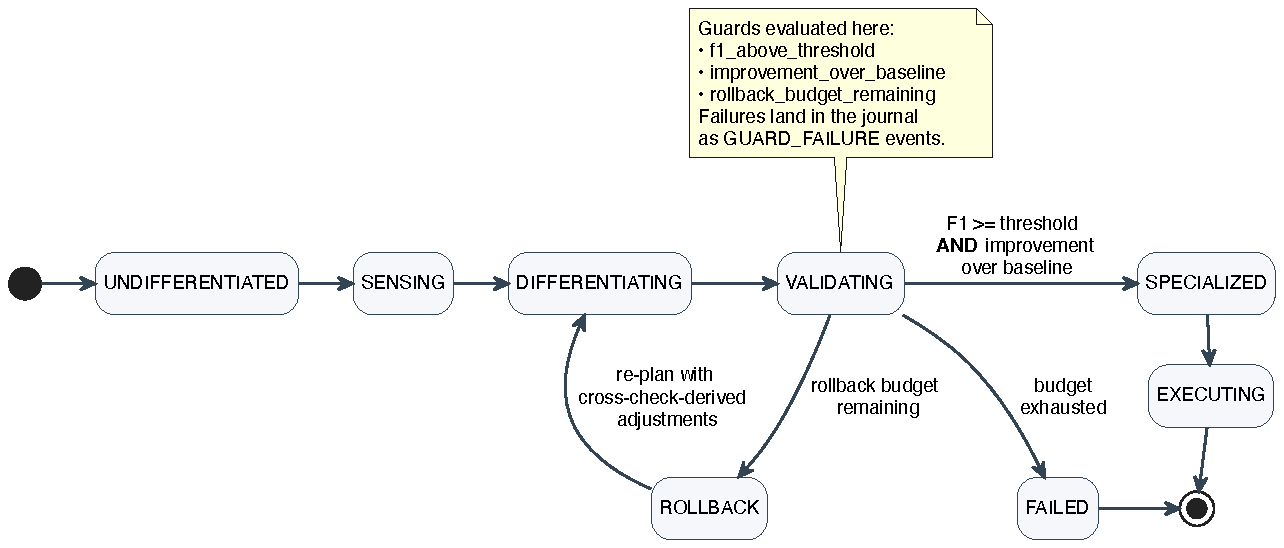
\includegraphics[width=0.88\linewidth]{state_machine.pdf}
    \caption{State machine with guarded transitions. Graduation to \texttt{SPECIALIZED} requires $F_1 \geq$ threshold and improvement over baseline. \texttt{ROLLBACK} re-enters \texttt{DIFFERENTIATING} carrying a diagnosis; \texttt{FAILED} is terminal when the rollback budget is exhausted.}
    \label{fig:state-machine}
\end{figure}

% =========================================================================
\section{Architecture}\label{sec:arch}

\paragraph{Enforced invariants} (see \figref{fig:components}) (i) \texttt{core/} and \texttt{phases/} import only from \texttt{ports/}. (ii) Agent state mutates only through \texttt{StateMachine.transition()}; guard predicates have signature \texttt{(context) -> (bool, reason)} and the reason lands in the journal. (iii) Every LLM call, metric, guard decision, capability registration, and state transition appends to the \texttt{EvolutionJournal}. (iv) All prompts flow through \texttt{compose\_system\_prompt()}; no ad-hoc strings elsewhere.

\paragraph{Capability registry and generation} Six hand-authored capabilities ship (\texttt{structural\_analysis}, \texttt{logic\_correctness}, \texttt{security\_analysis}, \texttt{performance\_analysis}, \texttt{style\_consistency}, \texttt{severity\_ranking}). Each declares a prompt fragment and optional static-tool references. Beyond them, the LLM proposes one novel capability per run. Generated Python passes an allowlist AST scan (forbidding \texttt{open}, \texttt{os}, \texttt{subprocess}, \texttt{\_\_import\_\_}, attribute access on blacklisted names) and then executes in a Python-isolated-mode subprocess bounded by \texttt{RLIMIT\_CPU} and a wall-clock timeout. Two independent layers, no external dependency. I chose this over \texttt{RestrictedPython} because the attack surface is auditable in under 60 lines. On the live run (\texttt{docs/example\_run/}) the proposal cleared both layers but planning did not select it, so the A/B below measures the composition-only path --- the sandbox is demonstrated, not load-bearing for the reported numbers.

\paragraph{Static-tool injection} \texttt{analyze\_structure} (AST metrics: max function length, max nesting depth) and \texttt{scan\_patterns} (regex: eval/exec on user input, SQL string concatenation, hardcoded credentials, \texttt{pickle.loads} of untrusted data) run before every specialized review. Their findings are injected into the prompt as a dedicated \texttt{Static Tool Findings} section. The undifferentiated baseline stays \emph{untooled}, so the A/B measures what self-specialization contributes, not what static analysis contributes.

\begin{figure}[!htbp]
    \centering
    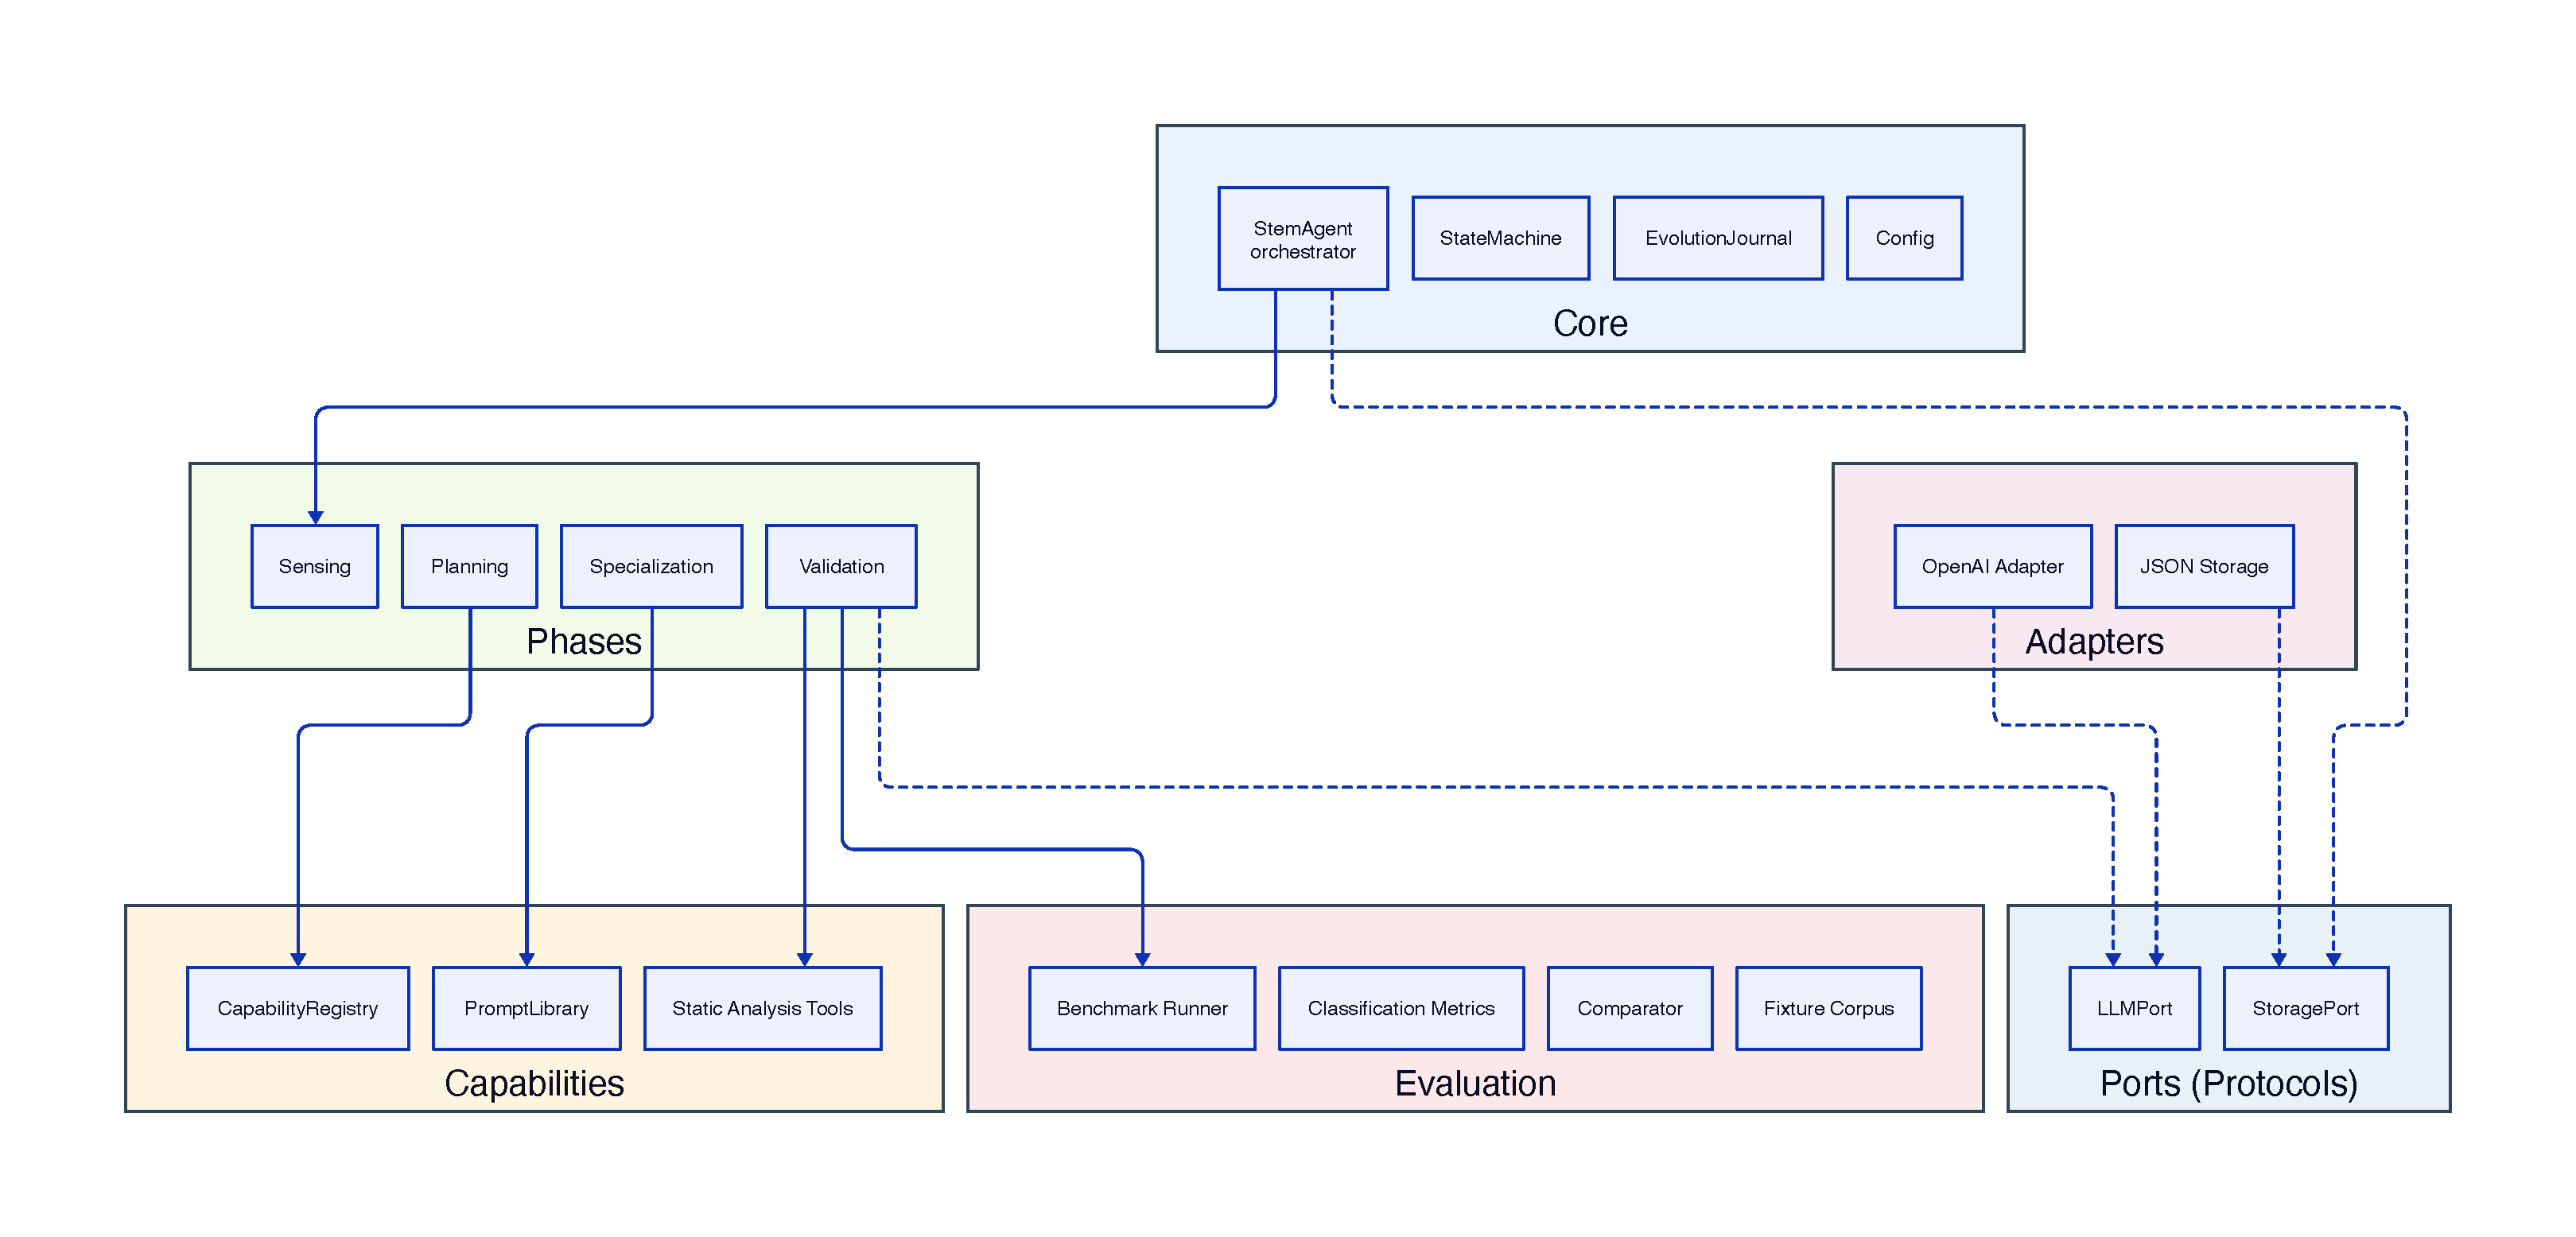
\includegraphics[width=\linewidth]{components.pdf}
    \caption{Component architecture. \texttt{core/} and \texttt{phases/} depend only on \texttt{LLMPort} and \texttt{StoragePort}. Every decision, metric, LLM call, guard result, and state transition appends to the \texttt{EvolutionJournal}: one log per run, one source of truth.}
    \label{fig:components}
\end{figure}

\paragraph{Phases} \emph{Sensing} asks the LLM for a structured domain profile (strategies, issue categories, tool categories, expert insights). \emph{Planning} consumes that profile and commits the capability set, the review-pass plan, and the $F_1$ / precision / recall thresholds that validation will enforce. \emph{Specialization} composes the system prompt; on a rollback retry, adjustments are spliced in under an \texttt{IMPORTANT adjustments based on prior evaluation} marker, so the specialization phase need not know a rollback happened. \emph{Validation} runs two benchmark passes (baseline and specialized) and a cross-check pass that replays every specialized verdict through the static tools, logging disagreements as \texttt{DECISION} events.

% =========================================================================
\section{Evaluation and rollback mechanism}\label{sec:eval}

\begin{table}[!htbp]
\small
\begin{tabularx}{\linewidth}{@{}lcX@{}}
\toprule
\textbf{Category} & \textbf{Count} & \textbf{Examples} \\
\midrule
Logic bugs & 5 & Off-by-one in binary search, wrong comparison operator, missing null check \\
Security & 4 & SQL injection via f-string, path traversal, hardcoded credentials, \texttt{eval()} on user input \\
Code smells & 4 & Deep nesting, god function, dead code after return, long parameter list \\
Performance & 2 & N+1 queries, unnecessary deep copy \\
Clean (adversarial) & 5 & Suspicious-looking but correct code; tests false-positive resistance \\
\bottomrule
\end{tabularx}
\captionsetup{skip=1pt}
\caption{Benchmark corpus of 20 labelled samples. Clean samples include code using \texttt{eval()} safely with \texttt{\_\_builtins\_\_=\{\}} and comparisons that look off-by-one but are correct for their domain.}
\end{table}

\paragraph{Test suite} 142 tests, zero network, under 4 seconds end-to-end. Hypothesis property tests search 200 random transition sequences per invariant (rollback monotonicity, \texttt{FAILED} terminality, guard-reason round-trip through the journal). \texttt{FakeLLM} is a first-class deterministic test double with substring-routed responses for every benchmark sample; \texttt{poor\_fake\_llm} returns degraded answers so the rollback branch is exercised with the same rigor as the happy path.

\paragraph{Metrics} A true positive is a buggy sample flagged with at least one issue in a ground-truth category; a true negative is a clean sample flagged with no issues. $F_1$ is the primary guard; specificity is tracked separately because it is the axis that decides false-positive resistance on the adversarial clean samples, and a high-$F_1$ reviewer with low specificity is still noise in practice.

\paragraph{Rollback diagnosis} When the graduation guard fails, \texttt{diagnose\_failure()} reads two signal sources. Benchmark deltas (precision / recall / specificity / $F_1$ direction) produce generic prompt nudges. Cross-check disagreements produce concrete adjustments: $N$ structure over-flags become ``do not flag structural problems unless a function exceeds $\sim$20 lines or depth exceeds 2''; $M$ scanner-caught security misses become ``scan harder for eval/exec on user input, hardcoded credentials, SQL string concatenation, \texttt{pickle.loads}'' with the exact patterns named. The adjustments are appended as a \texttt{ROLLBACK\_REASON} event and spliced into the next composed prompt. The next attempt is shaped by \emph{where} the last one went wrong, not just by how far $F_1$ fell short.

\begin{figure}[!htbp]
    \centering
    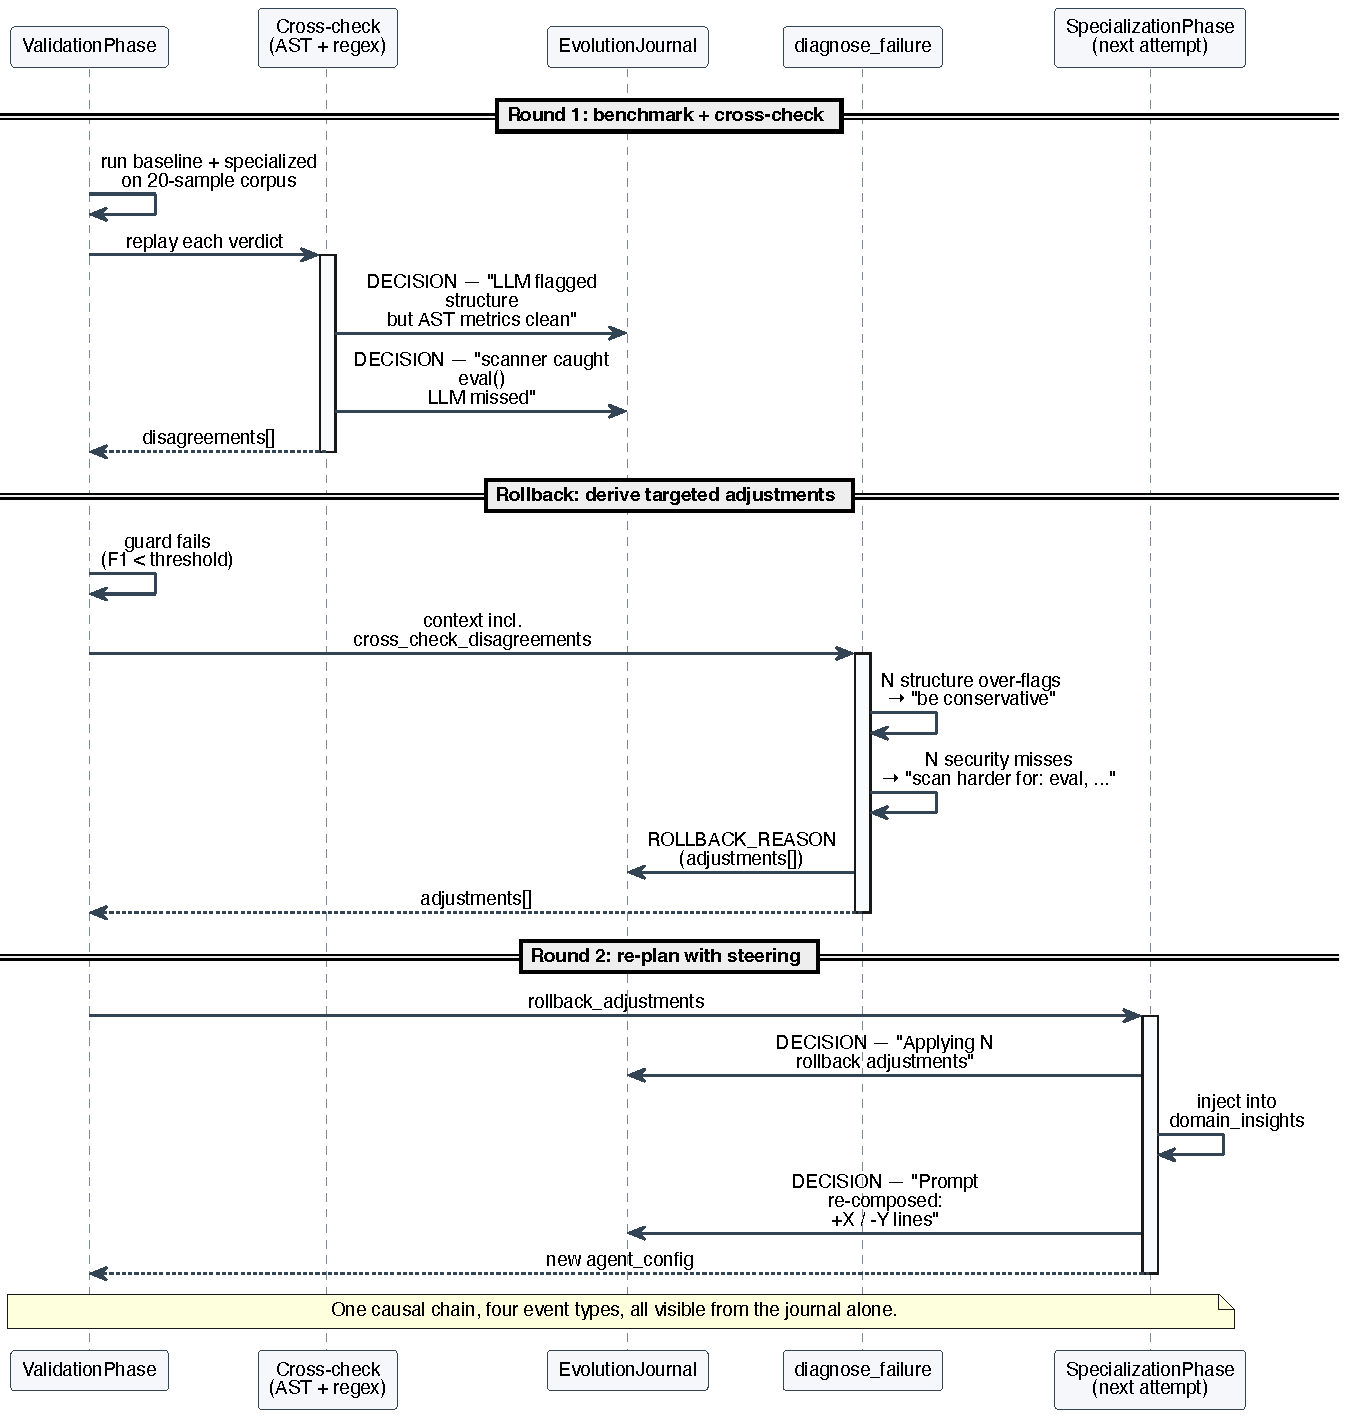
\includegraphics[width=0.82\linewidth]{feedback_loop.pdf}
    \caption{Closed feedback loop. Cross-check disagreements feed \texttt{diagnose\_failure()}, which emits concrete prompt adjustments that specialization splices into the next composition. Each edge writes a journal event, so the whole mechanism is auditable after the run.}
    \label{fig:feedback-loop}
\end{figure}

\paragraph{Results}

\begin{table}[!htbp]
\small
\centering
\begin{tabular}{@{}lcccc@{}}
\toprule
 & \textbf{Precision} & \textbf{Recall} & \textbf{$F_1$} & \textbf{Specificity} \\
\midrule
Baseline (undifferentiated, live) & 0.000 & 0.000 & 0.000 & 0.000 \\
Specialized (live OpenAI run) & 0.667 & 0.933 & \textbf{0.778} & 0.300 \\
\midrule
Rollback demo, attempt 1 (scripted) & 0.778 & 0.467 & 0.583 & 0.600 \\
Rollback demo, attempt 2 (scripted) & 1.000 & 1.000 & \textbf{1.000} & 1.000 \\
\bottomrule
\end{tabular}
\captionsetup{skip=1pt}
\caption{Live OpenAI run (\texttt{docs/example\_run/}): 42 LLM calls, $\sim$41k tokens, $\sim$\$0.20, no rollbacks triggered. Rollback demo (\texttt{docs/example\_run\_rollback/}) replays the same phase code against a scripted LLM boundary, exercising the $F_1$-fails-guard, diagnose, and re-specialize path the live run didn't trigger. Attempt 2's 1.0 is a property of the scripted fixture; 0.778 is the honest ceiling.}
\end{table}

The baseline zeros are a parser artefact, not a real ceiling. The undifferentiated prompt never asks for structured JSON, so the parser returns no categories on any sample, and precision and recall are undefined (they report as zero). Part of the specialization delta is bought by asking for JSON at all, not by deeper reasoning; nudging the baseline toward JSON would make the comparison ``fairer'', but output-structure discipline \emph{is} part of what specialization wins, so the honest framing leaves the numbers as they are. On the live run, the specialized pass catches 14 of 15 buggy samples (recall 0.933) while specificity sits at 0.300 on the five adversarial clean samples. The cross-check still surfaced three informational disagreements even though $F_1$ passed the guard, all logged as \texttt{DECISION} events for an auditor who wants to trace what the agent knows it is unsure about.

% =========================================================================
\section{Discussion}

\paragraph{Cross-check disagreements started as a score input} The first design penalized $F_1$ when the LLM disagreed with static analysis. That made validation stricter but taught the next attempt nothing. Feeding disagreements back as \emph{prompt guidance} is what actually closes the loop. Reframing from ``punish the score'' to ``shape the next attempt'' was the slowest insight of the project, and the one I am most glad I let the architecture survive.

\paragraph{Capability generation nearly didn't ship} Until late, the agent only \emph{selected} from the fixed registry, which is a composer, not a stem cell. Adding the sandboxed generation phase was the last meaningful change and the one that made the biological metaphor honest. The dual-layer defence (AST allowlist plus resource-limited subprocess) is belt-and-braces, but that is the right register for code an LLM wrote and the agent is about to run.

\paragraph{Specificity, not recall, is the axis that needs work} The live specialized pass catches 14 of 15 buggy samples but scores 0.300 on the adversarial clean corpus. That is \secref{sec:problem}'s corpus choice working: the five adversarial clean samples were designed to surface exactly this failure mode, an over-eager reviewer. The cross-check already caught two structural over-flags on this run without firing the graduation guard, both logged as \texttt{DECISION} events rather than papered over. A next iteration would weight the diagnoser harder on over-flag signals and grow the clean corpus so the ``be conservative on short functions'' adjustment has more evidence than a single heuristic.

\paragraph{With more time (and what I consciously cut)}
\begin{enumerate}[nosep]
  \item \emph{JSON-disciplined baseline.} The fair ablation: re-run the baseline with structured output requested, to separate what self-specialization buys from what output-format discipline alone buys. I expect the delta to shrink materially but stay positive.
  \item \emph{Second real domain.} The 8-sample security corpus is a first probe that the architecture generalizes, not a proof. A full second-domain live run is the natural next experiment.
  \item \emph{Multi-model evaluation.} \texttt{LLMPort} supports model overrides; a sweep would muddy the current A/B, which answers \emph{``does self-specialization beat an undifferentiated prompt''} honestly, but it is the next interesting question.
  \item \emph{Token-budget guard.} The journal totals tokens; no guard reads that total. Add it before anything user-facing, but not before a richer capability generator, because budget pressure only matters when attempt cost varies.
\end{enumerate}

\end{document}
